\section{Working with Result Sets}

The simulation apps produce result sets as output.
These are collections of result elements.
Result elements can be for example:
\begin{itemize}
\item Plain values: scalar or vector
\item Matrices
\item Charts
\item Images
\item Files
\item Tables
\end{itemize}

Result sets can be
\begin{enumerate}
\item stored in a file (extension *.isr),
\item displayed with a viewer program. A viewer is embedded into the workbench (tab "output") and a standalone viewer is available with the program \texttt{isResultTools}
\item or rendered into a PDF report.
\item In addition, with the \texttt{isResultTool}, comparisons between multiple result sets or extraction of selected elements can be done.
\end{enumerate}

\paragraph{Rendering of a Result Set}

Result sets are displayed in the "output" tab of the workbench.
When there are results displayed, those can be rendered or saved into an ISR file by selecting \menu{Results>Create Report...}

Whether a PDF report is rendered or a ISR file is written, depends on the file extension which is entered in the file dialog.

A report can also be rendered from a ISR file on disk.
Therefore the executable \texttt{isResultTool} exists. 
Once the program is started, select in the menu \menu{Results>Load...} and select the ISR file in the file selection dialog.
The result elements are then shown in the tree view on the left side of the window (\ref{fig:isresulttoolmainwindow}b).
To render the result elements into a PDF, select in the menu \menu{Results>Render...} and enter a file path to the desired output PDF file.
Optionally, some result set elements can be omitted from the PDF rendering by applying filters, see \ref{sec:resultsetfiltering}.


\begin{figure}[ht]
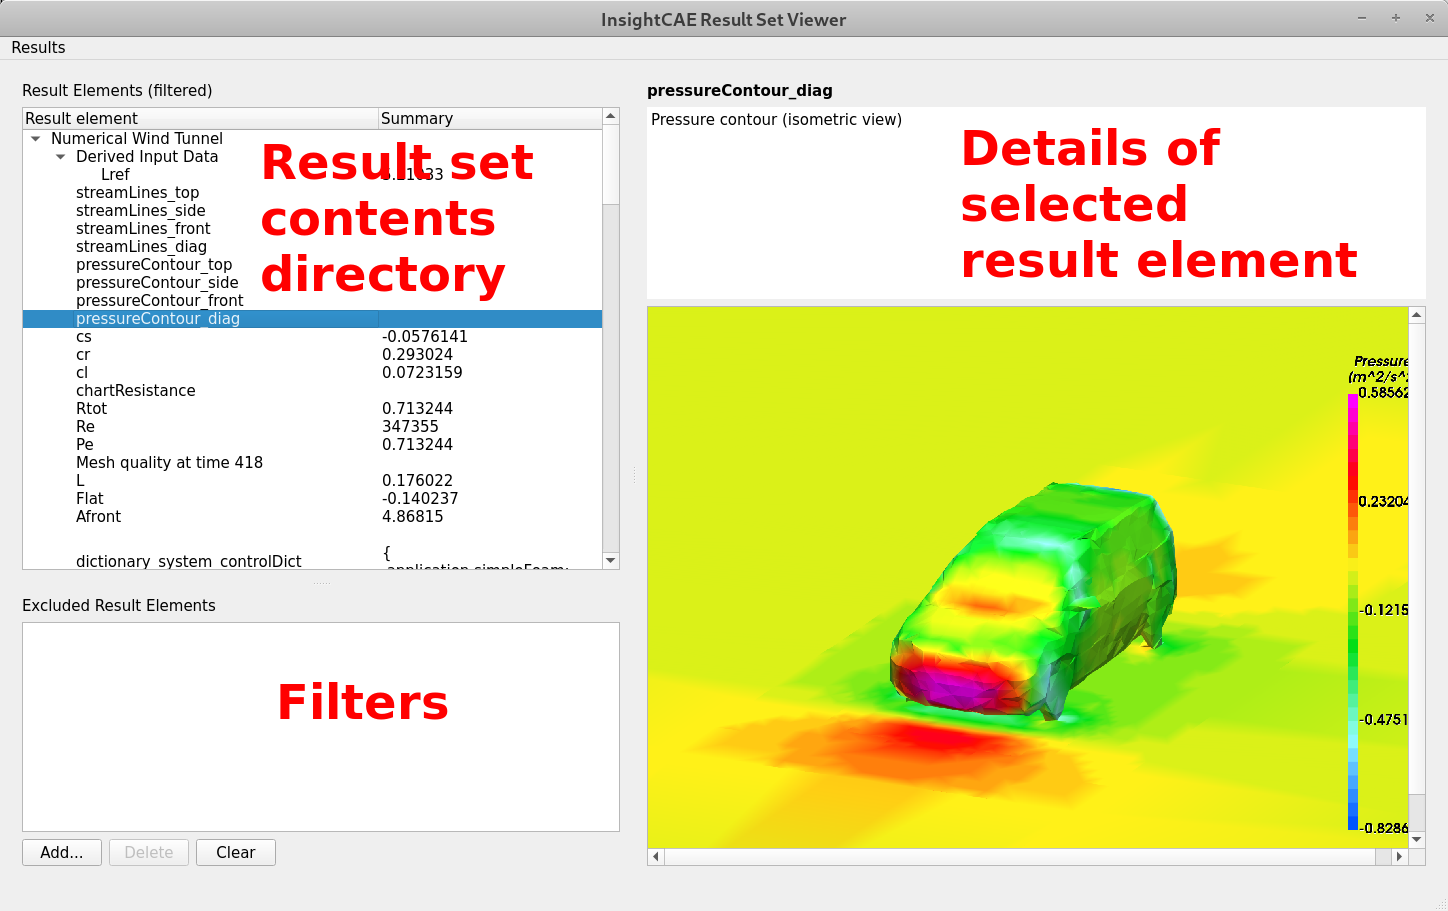
\includegraphics[width=\textwidth]{figs/isresulttool/InsightCAE_Result_Set_Viewer}
\caption{Main window of the \texttt{isResultTool}. a) bottom left: filters to be applied to the currently loaded result set, b) top left: content directory of the loaded result set (with the filters applied), c) right side: details of the result element that is selected in the top left tree view.}
\label{fig:isresulttoolmainwindow}
\end{figure}

Alternatively, the tool \texttt{isResultTool} can be executed with the command line argument \texttt{--render}:
\begin{lstlisting}
$ isResultTool --render savedResultset.isr
\end{lstlisting}



\paragraph{Applying Filters during Rendering}
\label{sec:resultsetfiltering}

A set of filters can be defined to render a report with some result elements excluded.
A filter is just a path-like text which represents the location of the result element in the result set hierarchy.
The concept is very similar to the specification of parameters, see section \ref{sec:parametersets} above.
Every result element, where the label path matches one of the filter expressions, is excluded.
The filter expressions, which are already defined, are shown in the list in the bottom left corner of the Result Set Viewer window, see figure \ref{fig:isresulttoolmainwindow}a.
The result set content directory, which is displayed in figure \ref{fig:isresulttoolmainwindow}b, shows the result set contents with all filters already applied.

To add filter expressions, click on the button "Add...".
The result element paths to filter out can be directly typed into the text field, one per line.
Instead of typing, result elements can be select from the full content of the result set after clicking the "..." button.

By default, a direct match of the entered text with the result element path is required.
Alternatively, the text entered in the input field can be treated as a regular expression\footnote{General informations: \url{https://en.wikipedia.org/wiki/Regular_expression}}\footnote{Syntax reference of the used parser:\\\url{https://www.boost.org/doc/libs/1_65_1/libs/regex/doc/html/boost_regex/syntax/perl_syntax.html}}.
If a regular expression was entered and shall be treated as such, the selection below the input field has to be changed to "regular expression".

Once a set of filter expressions is defined, it can saved to a file by selecting \menu{Results>Save filter...}.

Vice versa, a previously saved set of filter expressions can be loaded by \menu{Results>Load filter...}.

When the a report is rendered or saved into a ISR file, there is a switch on the bottom of the file dialog ("Save filtered result set").
This is by default checked.
If this is unchecked, the filter is skipped and the full report is rendered or saved.